\subsection{Slučaj upotrebe: Tehničke popravke}

\subsubsection*{Kratak opis}

Tehničko osoblje treba da zameni ili popravi stvari u pozorištu (zamena sijalice, farbanje, održavanje scene, itd.)

\subsubsection*{Akteri}
\begin{itemize}
    \item \textbf{Tehnički službenik} -- izvršava popravku
    \item \textbf{Finansijski službenik} -- proverava da li popravka ulazi u budžet i unosi nove troškove
    \item \textbf{Sistem} -- izvršava se automatski
\end{itemize}

\subsubsection*{Preduslovi}
\begin{itemize}
    \item Potrebno je izvršiti popravku ili zamenu potrošne robe u pozorištu.
\end{itemize}

\subsubsection*{Postuslovi}
\begin{itemize}
    \item Izmene su sačuvane.
\end{itemize}

\subsubsection*{Osnovni tok}
\begin{enumerate}
    \item Tehnički službenik je primetio da je potrebno izvršiti popravku.
    \item Tehnički službenik obaveštava finansijskog službenika o popravci i eventualnim troškovima.
    \item Finansijski službenik proverava da li popravka ne prelazi zadati budžet.
    \item Finansijski službenik odobrava popravku.
    \item Tehnički službenik izvršava popravku.
    \item Finansijski službenik unosi nove troškove u sistem.
    \item Sistem čuva nove izmene.
\end{enumerate}

\subsubsection*{Alternativni tokovi} 

\textbf{A1: Popravka prelazi budžet}
\begin{itemize}
    \item Finansijski službenik obaveštava tehničko osoblje da je budžet ispod granica troškova. Finansijski službenik stavlja u red popravki trenutnu popravku i slučaj se završava.
\end{itemize}

\subsubsection*{Specijalni zahtevi: /}

\subsubsection*{Dodatne informacije: /}

\begin{figure}[H]
	\centering
	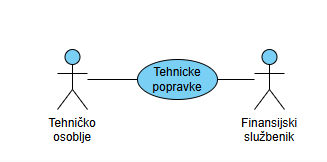
\includegraphics[width=\textwidth]{./Dijagrami/Dijagram slučajeva upotrebe/tehnicke_popravke.png} 
	\caption{Dijagram slučaja upotrebe "Tehničke popravke"}
\end{figure}

\begin{figure}[H]
    \centering
    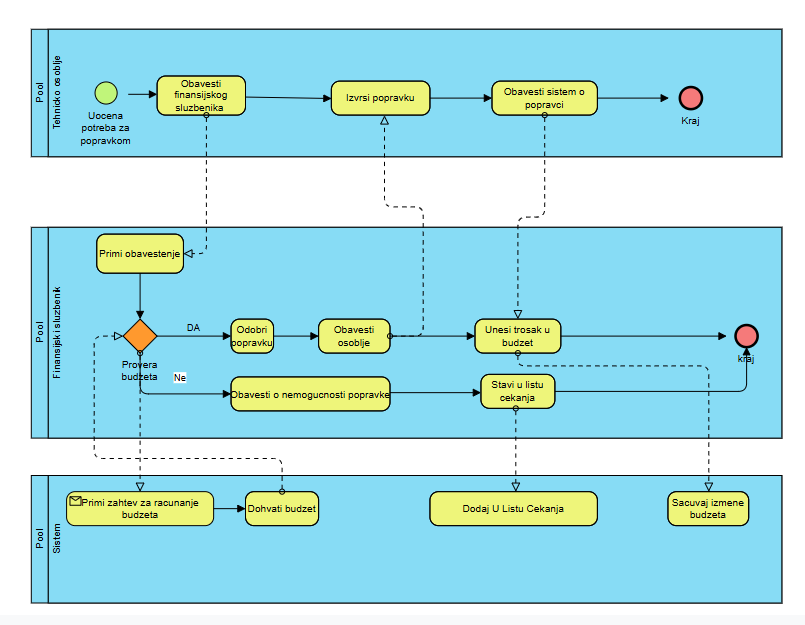
\includegraphics[width=\textwidth]{./Dijagrami/BPMN/tehnicke_popravke.png} 
    \caption{BPMN dijagram saradnje "Tehničke popravke"}
\end{figure}

\begin{figure}[H]
    \centering
    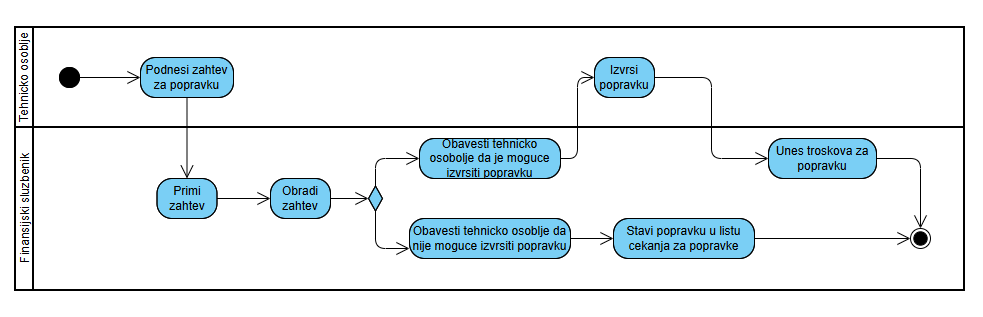
\includegraphics[width=\textwidth]{./Dijagrami/Dijagram aktivnosti/tehnicke_popravke.png} 
    \caption{Dijagram aktivnosti "Tehničke popravke"}
\end{figure}

\begin{figure}[H]
    \centering
    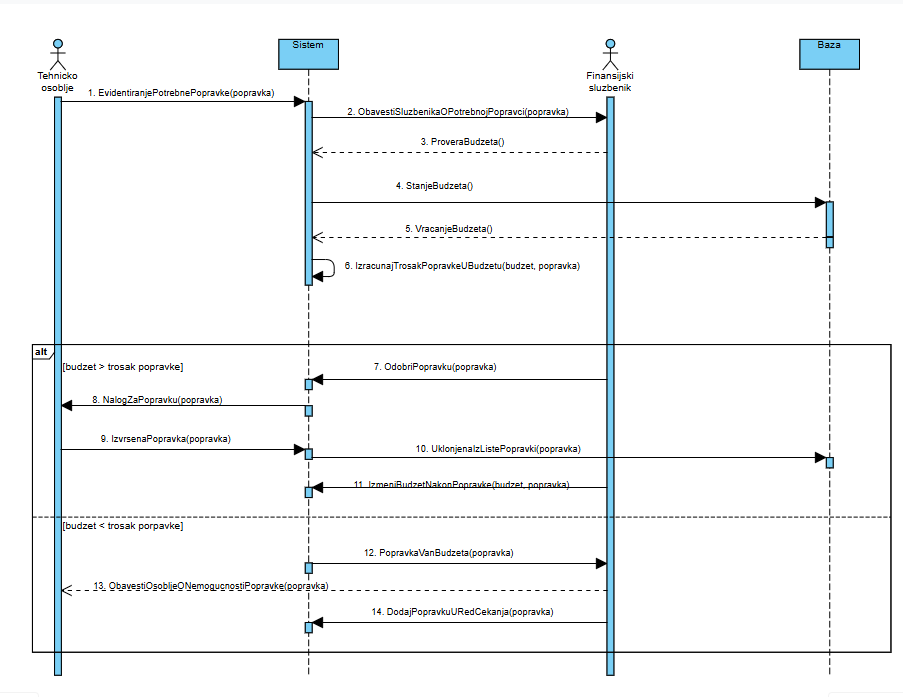
\includegraphics[width=\textwidth]{./Dijagrami/Dijagram sekvence/tehnicke_popravke.png} 
    \caption{Dijagram sekvence "Tehničke popravke"}
\end{figure}

\newpage